\documentclass[journal, a4paper]{IEEEtran}

\usepackage{amsmath}     
\usepackage{graphicx}
\usepackage{url}       
%\usepackage{cite}   
%\usepackage{psfrag} 
%\usepackage{subfigure}
%\usepackage{stfloats}
%\usepackage{array}

\begin{document}
% Define document title and author
	\title{Gene expression patterns distinguish breast carcinomas from normal breast tissues}
	\author{Ilia Abolhasani}
	\markboth{Introduction to Bioinformatics at Sharif university of technology}{}
	\maketitle

% Write abstract here
\begin{abstract}
	Genomic alterations can change cellular processes and make differentiation in gene expression and make cancer. In this project aims to use statistical analysis for determine and specify up-regular and down-regular genes by significantly distinct between normal and breast cancer in Malays, Chinese and Indians people. We used micro-array data sets with GSE number 15852 that included 43 breast cancer and 43 normal samples.
\end{abstract}

\section{Introduction}
	\PARstart{B}{reast} cancer is a cancer that forms in the cells of the breasts and the most common cancer diagnosed in women.
    \\Used Affy-metrix  \textit{U133A} Gene-Chips that containing 22,283 probe sets targeting 18,400 different transcripts with platform number  \textit{GPL96} to collect the data used in this project.
    \\The data set is available for download with \textit{GSE15852} number in  \textit{NCBI} and include 43 breast carcinomas and 43 patient-matched normal tissues.
    For statistical analysis use  \textit{R language} and  \textit{Enrichr} website.
\section{Code explanation}
	In the first step, we use \textit{GEOquery} library and download data set with \textit{GSE15852} number and \textit{GPL96} platform number. Then, made 2 groups and tagged data to this groups. (G0 = normal, G1 = cancer).
	\\Since the value of genetic expression is high, it is turned to logarithmic space and according to the seen box-plot \figurename{\ref{fig:boxplot}}it was made normalized\figurename{\ref{fig:boxplot_norm}}.
	Then, we used Limma package to fit a linear model between G1 and G0 groups and Bayesian model started with 0.01 hypothesis value for the amount of genes that has changed.
	\\So, p-value was calculated for 2 groups and p-value was adjusted
	 with Benjamini–Hochberg false discovery rate method.
	After that, we made two sets, up-regular and down-regular by thresholding.
	\\down-regular was made by adjusted p-value lower than 0.05 and logFC (log for change) lower than -1.
	up-regular was made by adjusted p-value lower than 0.05 and logFC greater
	than 1.
	we passed up-regular and down-regular gene list to Enrichr website and found genes that significantly involved in regular transcription in cell process.
	\section{Conclusion}
    This present study found genetic changes that significantly involve in breast cancer. Base on results, some genes act as trigger to other genes and with finding this genes, cancer can be cured by suppressing this genes by drug. if any drug is design to suppress RXRA gene or NFYB gene, then we can prevent cell to become cancer cell.
    For future studies, we can use machine learning algorithms and use this significant gene as feature for classification between normal and cancer samples. for example, ANFIS (Adaptive neuro fuzzy inference system) with considering significant gene as membership functions can be a good method for apply to this purpose.
	\section{Tables and Figures}
    \begin{table}[!hbt]
		\begin{center}
		\caption{TRANSFAC and JASPAR PWMs}
		\label{tab:simParameters}
		\begin{tabular}{
		|c|c|c|c|c|c|}
			\hline
			Name & Adjusted p-value & Z-score & Combined score\\
			\hline
			RXRA (human) & 0.005396 & -1.76	& 18.99\\
			\hline
            NFYB (human) & 0.2042	& -2.42 &14.65\\
            \hline
            ESR1 (human) & 0.2042	& -1.78 & 11.23\\
            \hline
            TFAP2C (human) & 0.7907	& -1.66 & 7.36\\
            \hline
            HIF1A (human) & 0.9999	& -1.70	& 6.35\\
			\hline
		\end{tabular}
		\end{center}
	\end{table}
	
	\begin{table}[!hbt]
		\begin{center}
		\caption{Reactome 2016}
		\label{tab:simParameters}
		\begin{tabular}{
		|p{3cm}|c|c|c|}
			\hline
			Name & Adjusted p-value & Z-score & Combined score\\
			\hline
            Cell Cycle, Mitotic_Homo sapiens_R-HSA-69278 & 0.002174 & -2.48	& 30.97\\
            \hline
	        Cell Cycle_Homo sapiens_R-HSA-1640170 &	0.003502 & -2.45	& 27.79\\
	        \hline
            DNA Replication_Homo sapiens_R-HSA-69306 &	0.005111 & -2.28 & 23.01\\
            \hline
		\end{tabular}
		\end{center}
	\end{table}
	
	
	\begin{figure}[!hbt]
		\begin{center}
		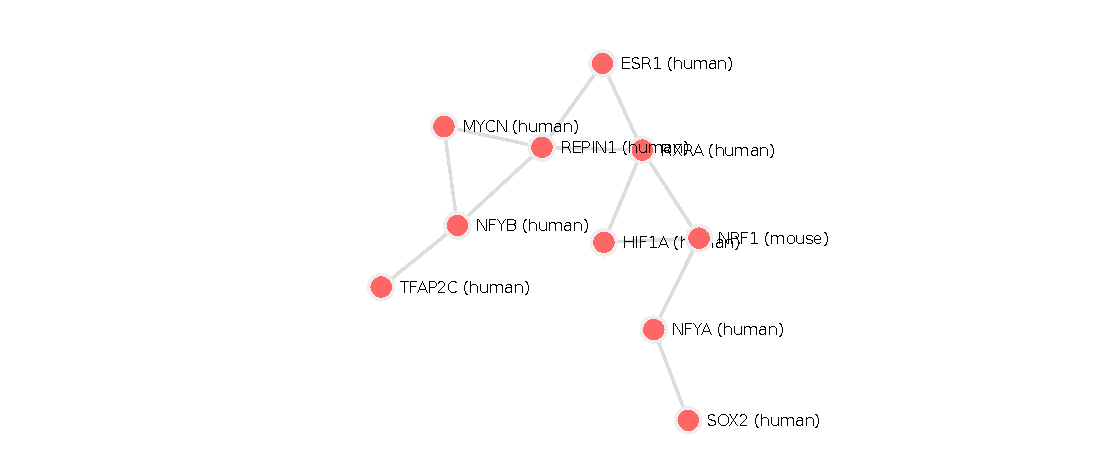
\includegraphics[width=\columnwidth]{network}
		\caption{TRANSFAC and JASPAR PWMs Network}
		\label{fig:network}
		\end{center}
	\end{figure}
	
	\begin{figure}[!hbt]
		\begin{center}
		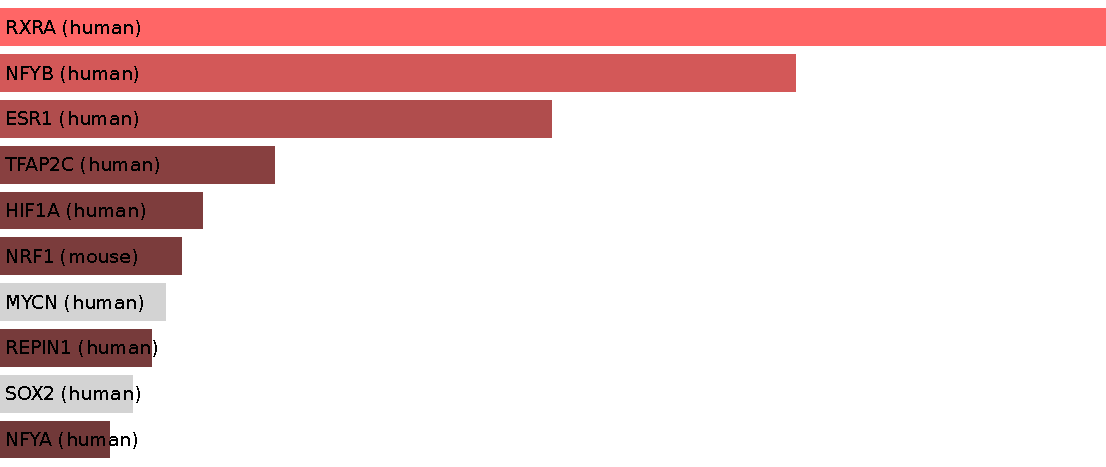
\includegraphics[width=\columnwidth]{bar-graph.pdf}
		\caption{TRANSFAC and JASPAR PWMs Bar graph}
		\label{fig:Bar-Graph}
		\end{center}
	\end{figure}
	
	\begin{figure}[!hbt]
		\begin{center}
		
\includegraphics[width=\columnwidth]{boxplot.pdf}
		\caption{box plot for data }
		\label{fig:boxplot}
		\end{center}
	\end{figure}
	
	\begin{figure}[!hbt]
		\begin{center}
		
\includegraphics[width=\columnwidth]{boxplot_norm.pdf}
		\caption{box plot for data after normalize}
		\label{fig:boxplot_norm}
		\end{center}
	\end{figure}
	
	\begin{figure}[!hbt]
		\begin{center}
		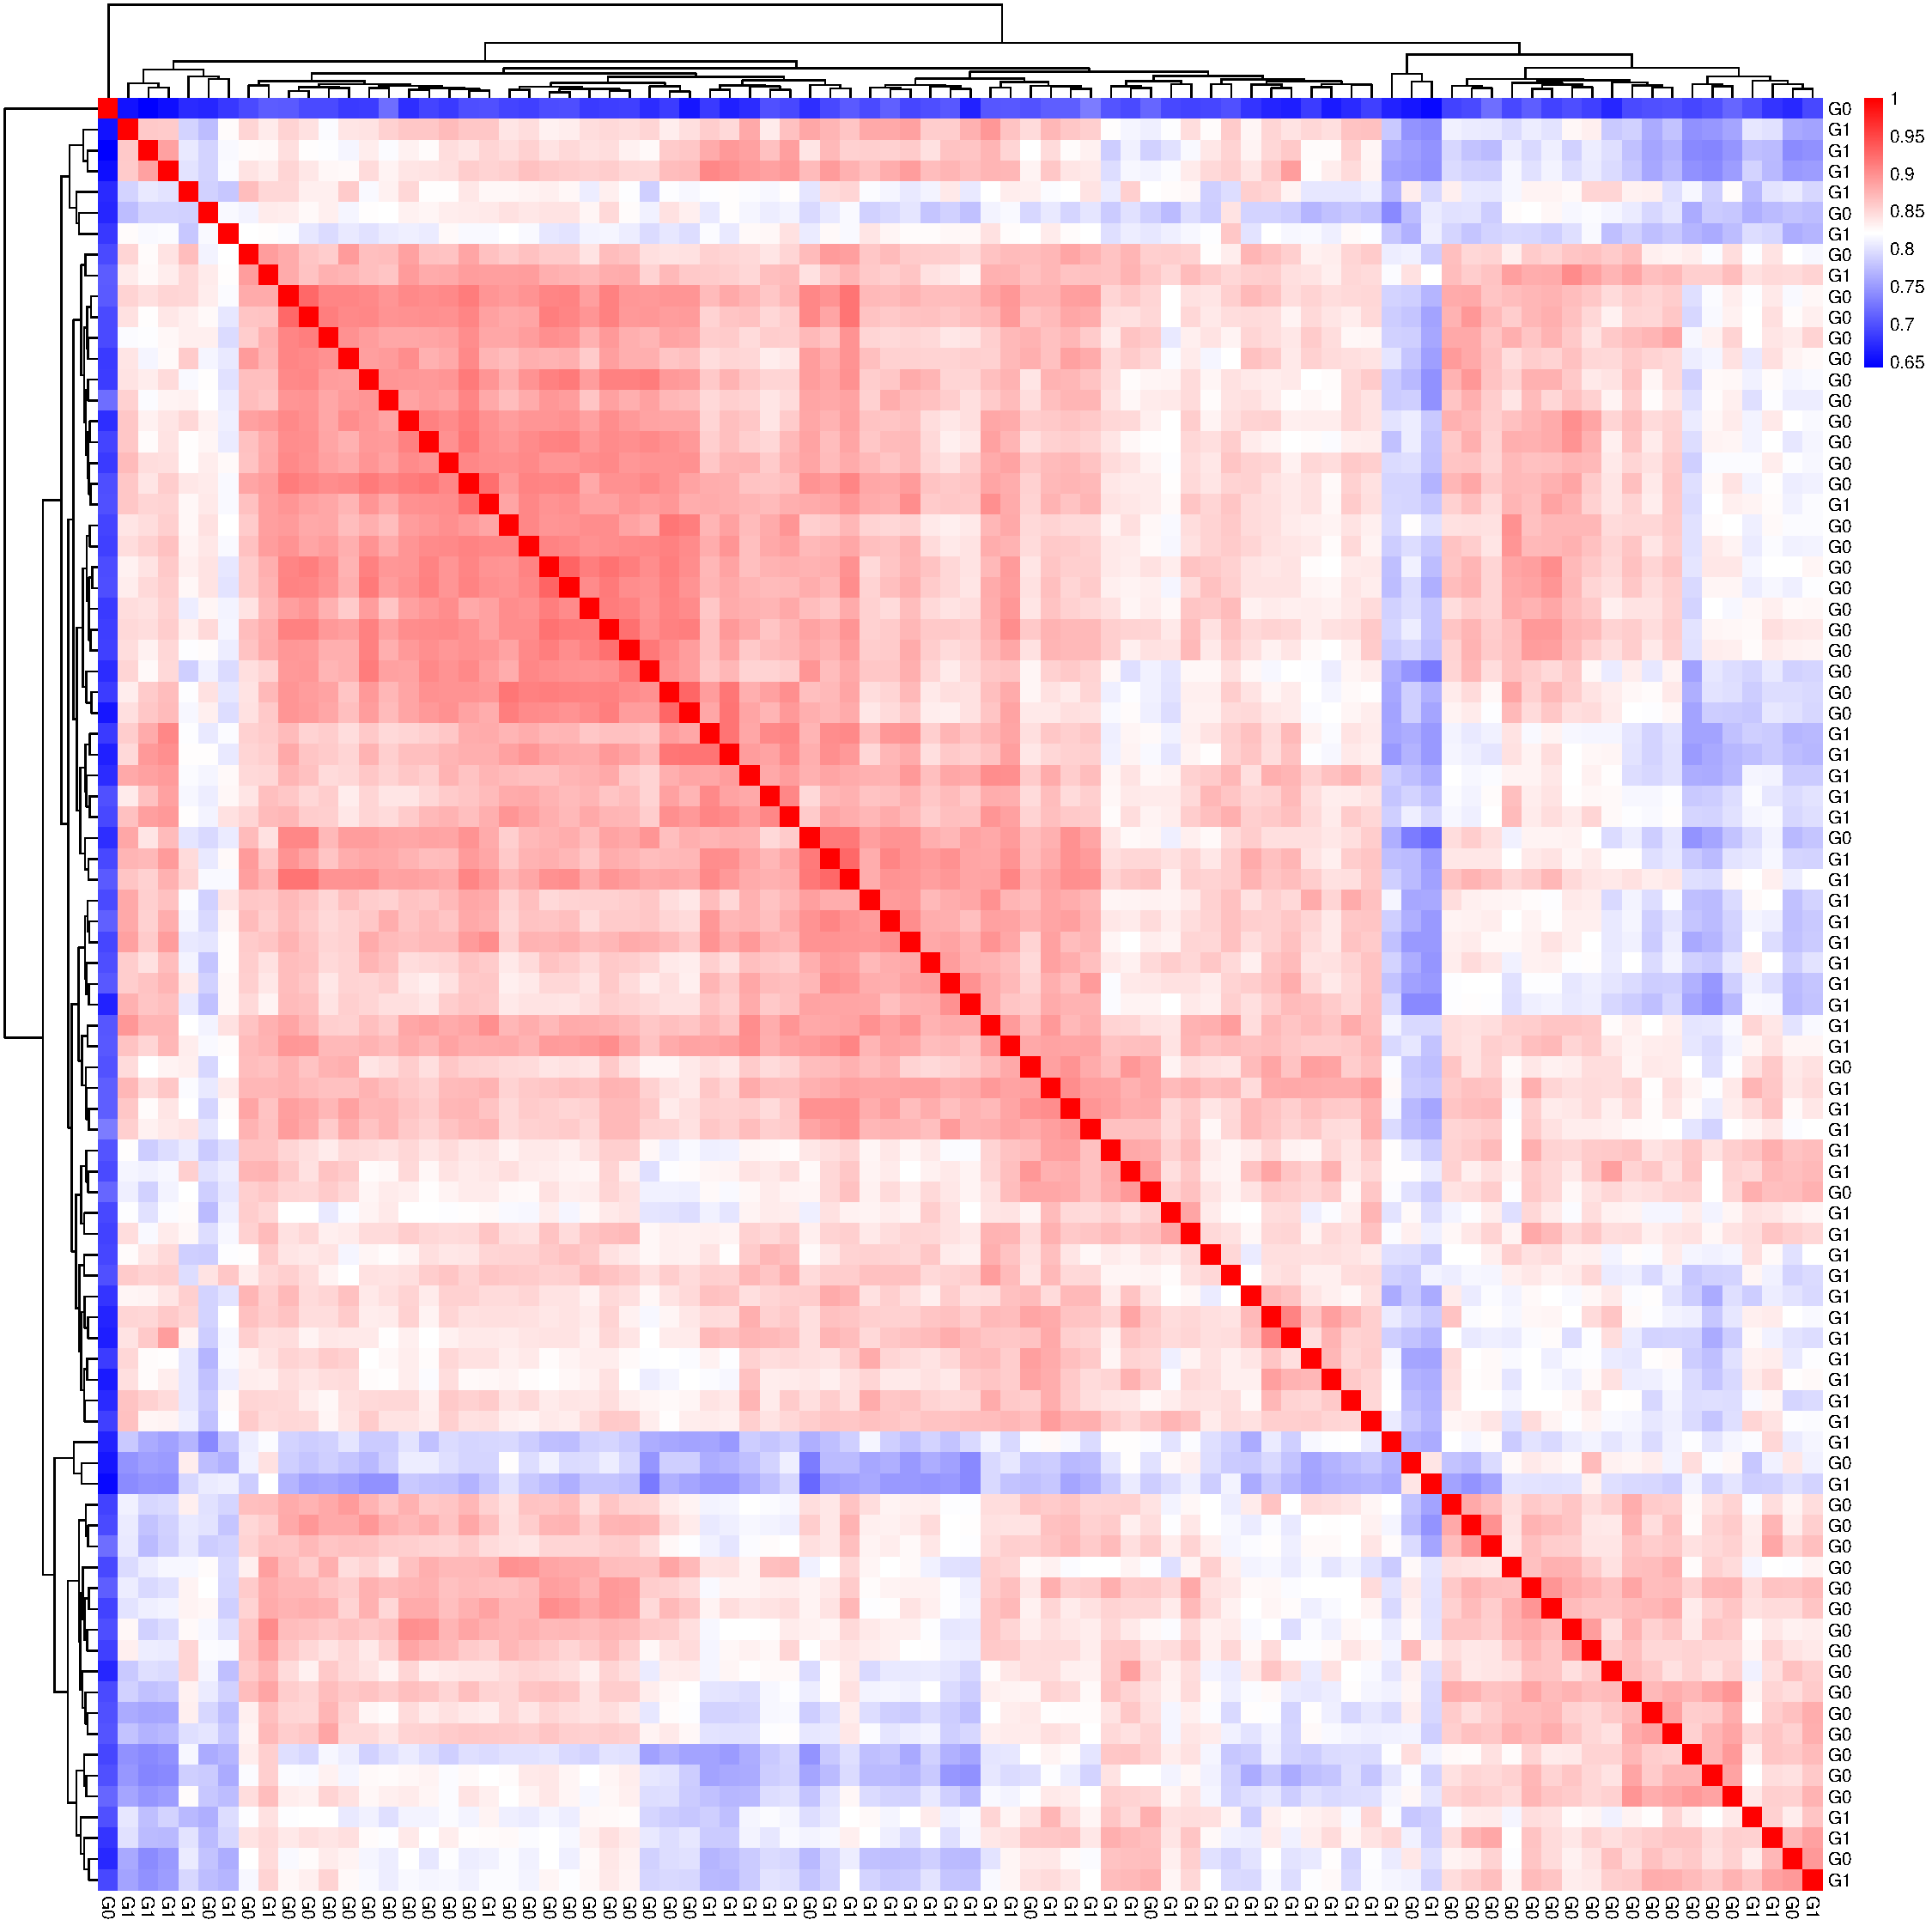
\includegraphics[width=\columnwidth]{CorHeatmap.pdf}
		\caption{Correlation Heatmap between 86 samples}
		\label{fig:network}
		\end{center}
	\end{figure}
	
	\begin{figure}[!hbt]
		\begin{center}
		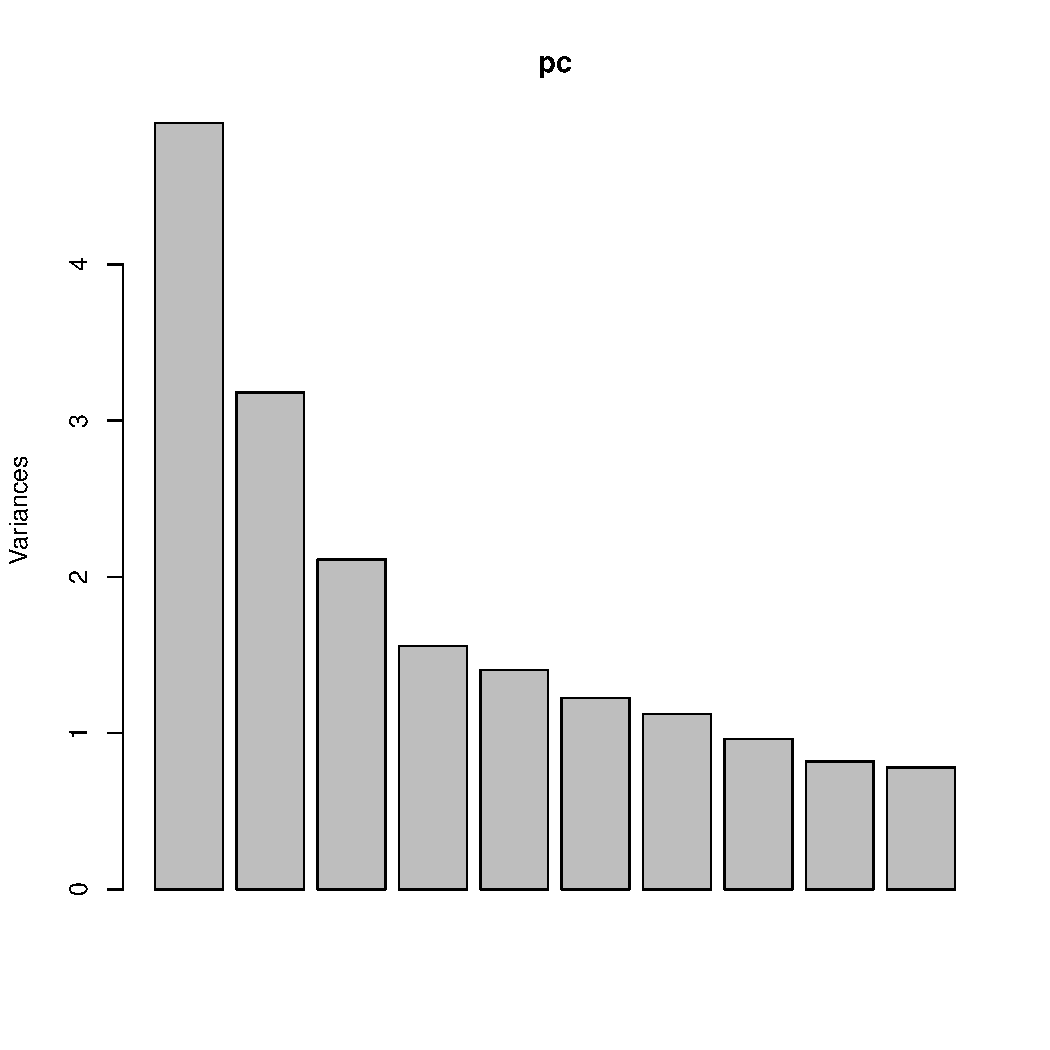
\includegraphics[width=\columnwidth]{pca.pdf}
		\caption{Principal component analysis}
		\label{fig:network}
		\end{center}
	\end{figure}
\end{document}